\documentclass[letterpaper, headinclude, footinclude = true]{article}
\usepackage{tikz}
\PassOptionsToPackage{noopticals}{MinionPro}
\usepackage[minionprospacing, nochapters, beramono, listings, minionpro]{classicthesis}
\usepackage{amsmath}
\usepackage{graphicx}
\usepackage{float}
\usepackage{listings}

\lstset{language=[LaTeX]Tex,%C++,
    keywordstyle=\color{RoyalBlue},%\bfseries,
    basicstyle=\small\ttfamily,
    %identifierstyle=\color{NavyBlue},
    commentstyle=\color{Green}\ttfamily,
    stringstyle=\rmfamily,
    numbers=none,%left,%
    numberstyle=\scriptsize,%\tiny
    stepnumber=5,
    numbersep=8pt,
    showstringspaces=false,
    breaklines=true,
    frameround=ftff,
    %frame=single,
    belowcaptionskip=.75\baselineskip
    %frame=L
} 

\usetikzlibrary{intersections}


\begin{document}

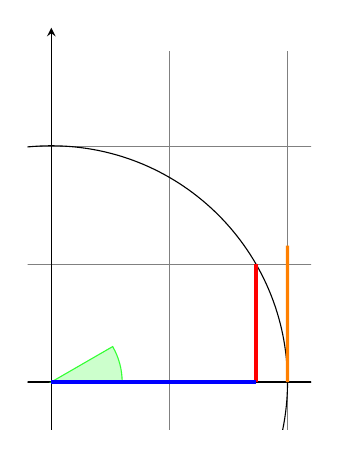
\begin{tikzpicture}[scale = 3, >=stealth],
\clip (-0.1, -0.2) rectangle (1.1, 1.5);
\draw [help lines, step = 0.5cm] (-1.4, -1.4) grid (1.4, 1.4);
\draw [->] (-1.5,0) -- (1.5, 0);
\draw [->] (0, -1.5) -- (0, 1.5);
\draw (0,0) circle [radius = 1 cm];

\filldraw[fill = green!20, draw = green!80] 
	(0,0) -- (0.3, 0) arc [start angle = 0, end angle = 30, radius = 3 mm] -- cycle;

\draw [red, very thick] (30:1)	-- +(0, -0.5);
\draw [blue, very thick] (30:1 |- 0,0) -- (0,0);

\path [name path = upward line] (1,0) -- (1,1);
\path [name path = slanted line] (0,0) -- (30:2);
\draw [name intersections = {of = upward line and slanted line, by = x}] [very thick, orange] (1,0) -- (x);



\end{tikzpicture}





\end{document}